%!TEX root=../../autopilot.tex
\begin{figure*}[ht!]
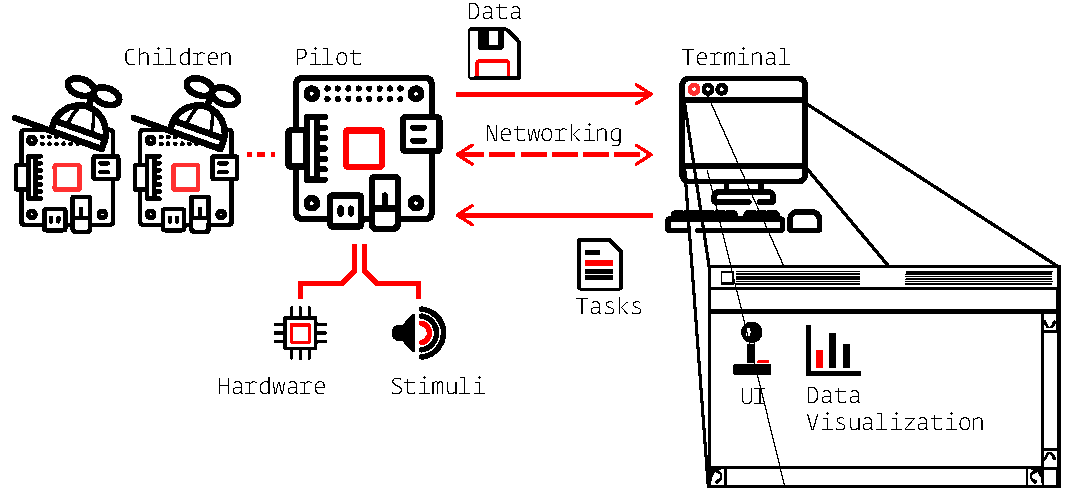
\includegraphics[width=\linewidth+\marginparsep+\marginparwidth]{autopilot/autopilot/src/figures/whole_system_black.pdf}
\caption{Overview of major Autopilot components}
\end{figure*}

\newthought{Autopilot consists of software and hardware modules}\break configured to create a behavioral \hyperref[sec:topology]{topology}. Independent \hyperref[sec:agents]{agents} linked by flexible \hyperref[sec:networking]{networking} objects fill different roles within a topology, such as hosting the \hyperref[sec:ui]{user interface}, controlling \hyperref[sec:hardware]{hardware}, \hyperref[sec:transforms]{transforming} incoming and outgoing data, or delivering \hyperref[sec:stim]{stimuli}. This infrastructure is ultimately organized to perform a behavioral \hyperref[sec:tasks]{task}.